\documentclass[aspectratio=169,11pt]{beamer}
\usepackage[T1]{fontenc}
\usepackage{lmodern}
\usepackage{amsmath,amssymb,booktabs,listings}
\usetheme{Madrid}
\usecolortheme{dolphin}
\setbeamertemplate{blocks}[rounded][shadow=false]
\definecolor{Navy}{HTML}{15345C}
\definecolor{Teal}{HTML}{2266B3}
\definecolor{Coral}{HTML}{D6603C}
\definecolor{Mist}{HTML}{EFF5FC}
\setbeamercolor{normal text}{fg=Navy,bg=white}
\setbeamercolor{structure}{fg=Teal}
\setbeamercolor{frametitle}{fg=white,bg=Navy}
\setbeamercolor{title}{fg=white,bg=Navy}
\setbeamercolor{subtitle}{fg=white}
\setbeamercolor{alerted text}{fg=Teal}
\setbeamercolor{palette primary}{fg=white,bg=Teal}
\setbeamercolor{palette secondary}{fg=white,bg=Navy}
\setbeamercolor{palette tertiary}{fg=white,bg=Navy}
\setbeamercolor{block title}{fg=white,bg=Teal}
\setbeamercolor{block body}{fg=Navy,bg=Mist}
\setbeamerfont{title}{size=\Huge,series=\bfseries}
\setbeamerfont{frametitle}{size=\Large,series=\bfseries}
\setbeamertemplate{navigation symbols}{}
\setbeamertemplate{itemize items}[circle]
\setbeamersize{text margin left=9mm,text margin right=9mm}
\setbeamertemplate{headline}{}
\setbeamertemplate{footline}{%
 \leavevmode\hbox{%
 \begin{beamercolorbox}[wd=.84\paperwidth,ht=2.8ex,dp=1.2ex,leftskip=9mm]{palette secondary}%
 \scriptsize DRP\enspace\textbar\enspace Neural Network Learning
 \end{beamercolorbox}%
 \begin{beamercolorbox}[wd=.16\paperwidth,ht=2.8ex,dp=1.2ex,center]{palette primary}%
 \scriptsize\insertframenumber\,/\,\inserttotalframenumber
 \end{beamercolorbox}}}
\lstset{language=Python,basicstyle=\ttfamily\small,keywordstyle=\color{Teal}\bfseries,
 stringstyle=\color{Coral},showstringspaces=false,columns=fullflexible,keepspaces=true,
 frame=none,backgroundcolor=\color{Mist},xleftmargin=2mm,xrightmargin=2mm,
 aboveskip=3mm,belowskip=3mm,breaklines=false}
\newcommand{\source}{\vfill{\tiny\color{gray}PyTorch: \href{https://docs.pytorch.org/tutorials/beginner/basics/optimization_tutorial.html}{Optimizing Model Parameters}}}
\title{Learning a function\\with a neural network}
\subtitle{A first example: \texorpdfstring{$\sin(x)$ on $[0,\pi]$}{sin(x) on [0, pi]}}
\author{Directed Reading Program}
\date{}
\begin{document}

\begin{frame}
\titlepage
\vspace{-5mm}
\centering\textcolor{Teal}{Data \quad Architecture \quad Loss \quad Training \quad Testing}
\end{frame}

\begin{frame}{A neural network is a family of functions}
\large
\[\boxed{\widehat y=f_\theta(x)}\]
\begin{itemize}\setlength\itemsep{4mm}
\item $x$ is an input and $\widehat y$ is the predicted output.
\item $\theta$ collects the adjustable \alert{weights and biases}.
\item The architecture tells us how to combine these parameters.
\item Learning means choosing $\theta$ so predictions fit examples.
\end{itemize}
\vspace{3mm}
Today: one real input, one real output, and a known target $y=\sin(x)$.
\end{frame}

\begin{frame}{Inside one hidden neuron}
\begin{columns}[c]
\begin{column}{0.47\textwidth}
\Large
\[z=wx+b\]
\[h=\tanh(z)\]
\normalsize
For example, if $w=2$, $b=-1$, and $x=0.5$, then $z=0$ and $h=0$.
\end{column}
\begin{column}{0.48\textwidth}
\begin{itemize}\setlength\itemsep{4mm}
\item The weight $w$ scales the input.
\item The bias $b$ shifts the response.
\item The activation $\tanh$ introduces a nonlinear shape.
\end{itemize}
\end{column}
\end{columns}
\vspace{7mm}
\textcolor{Teal}{Training changes $w$ and $b$. The activation formula stays fixed.}
\end{frame}

\begin{frame}{Our network has 49 trainable parameters}
\large
\[h_j(x)=\tanh(w_jx+b_j),\qquad j=1,\ldots,16\]
\[\boxed{f_\theta(x)=c+\sum_{j=1}^{16}v_jh_j(x)}\]
\vspace{2mm}
\normalsize
\begin{center}
\begin{tabular}{lrl}
\toprule
Part & Parameters & Meaning\\\midrule
Input to hidden layer & $16+16$ & Weights $w_j$ and biases $b_j$\\
Hidden to output layer & $16+1$ & Weights $v_j$ and bias $c$\\\midrule
Total & $49$ & Numbers adjusted during training\\\bottomrule
\end{tabular}
\end{center}
\vspace{2mm}
The output is a weighted sum of 16 learned nonlinear responses.
\end{frame}

\begin{frame}{Why the activation matters}
\large
If we remove $\tanh$, the network becomes
\begin{align*}
f_\theta(x)&=c+\sum_{j=1}^{16}v_j(w_jx+b_j)\\[2mm]
&=\underbrace{\left(\sum_jv_jw_j\right)}_{A}x
+\underbrace{\left(c+\sum_jv_jb_j\right)}_{B}.
\end{align*}
\vspace{3mm}
This is still a straight line: $Ax+B$.
\vspace{4mm}

\textcolor{Teal}{Nonlinear activations let the network represent curved functions.}
\end{frame}

\begin{frame}[fragile]{1. Training data}
\begin{columns}[c]
\begin{column}{0.46\textwidth}
\begin{lstlisting}[basicstyle=\ttfamily\footnotesize]
import torch
from torch import nn

torch.manual_seed(7)
x_train = torch.linspace(
    0, torch.pi, 64
).reshape(-1, 1)
y_train = torch.sin(x_train)
\end{lstlisting}
\small
64 equally spaced inputs, including $0$ and $\pi$. All angles use radians.
\vspace{3mm}

Shape \texttt{(64, 1)}: 64 examples with one input feature each.
\end{column}
\begin{column}{0.53\textwidth}
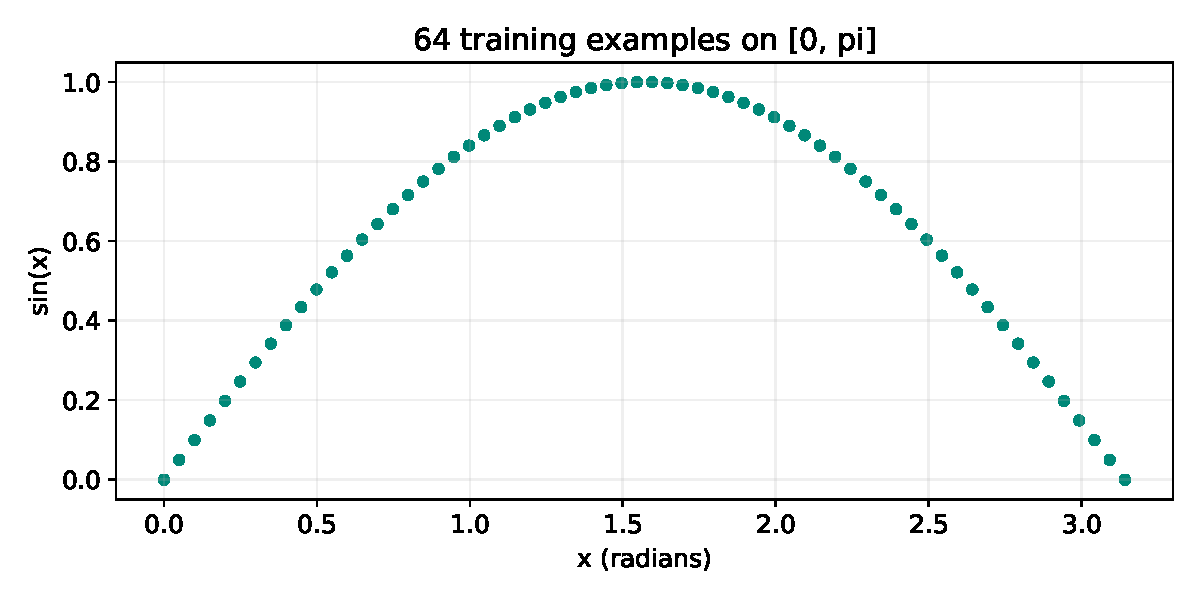
\includegraphics[width=\linewidth]{figures/training_data.pdf}
\end{column}
\end{columns}
\end{frame}

\begin{frame}[fragile]{2. Architecture in PyTorch}
\begin{columns}[c]
\begin{column}{0.49\textwidth}
\begin{lstlisting}
model = nn.Sequential(
    nn.Linear(1, 16),
    nn.Tanh(),
    nn.Linear(16, 1)
)
\end{lstlisting}
\end{column}
\begin{column}{0.46\textwidth}
\begin{tabular}{ll}
\toprule
Operation & Batch shape\\\midrule
Input & $64\times 1$\\
First linear layer & $64\times16$\\
Activation & $64\times16$\\
Output layer & $64\times 1$\\\bottomrule
\end{tabular}
\end{column}
\end{columns}
\vspace{7mm}
PyTorch initializes the weights and biases. They do not yet fit the data.
\vspace{3mm}

\texttt{Tanh} has no trainable parameters. The final layer has no activation.
\end{frame}

\begin{frame}[fragile]{3. Loss: mean squared error}
\large
\[L(\theta)=\frac{1}{64}\sum_{i=1}^{64}\bigl(f_\theta(x_i)-y_i\bigr)^2\]
\normalsize
\begin{lstlisting}
loss_fn = nn.MSELoss()
\end{lstlisting}
\begin{itemize}\setlength\itemsep{3mm}
\item Subtract the target from each prediction.
\item Square each difference, then take the average.
\item A smaller loss means closer agreement on these examples.
\end{itemize}
\vspace{3mm}
Zero training loss would mean matching all 64 training targets exactly.
\source
\end{frame}

\begin{frame}{Backpropagation is the chain rule}
For one example, let $e=f_\theta(x)-y$, $\ell=e^2$, and $h_j=\tanh(w_jx+b_j)$.
\vspace{3mm}
\large
\[\frac{\partial\ell}{\partial v_j}=2e\,h_j\]
\[\frac{\partial\ell}{\partial w_j}
=\underbrace{2e}_{\text{output error}}
\underbrace{v_j}_{\text{output weight}}
\underbrace{(1-h_j^2)}_{\tanh\text{ derivative}}
\underbrace{x}_{\text{input}}\]
\normalsize
\vspace{4mm}
The derivative tells us how a small parameter change affects the loss.
\vspace{3mm}

For MSE, average these derivatives over the training examples.\\
\texttt{loss.backward()} calculates them automatically for all parameters.
\vfill{\tiny\color{gray}PyTorch: \href{https://docs.pytorch.org/tutorials/beginner/basics/autogradqs_tutorial.html}{Automatic Differentiation}}
\end{frame}

\begin{frame}[fragile]{Gradient descent adjusts the parameters}
\large
\[\boxed{\theta_{\mathrm{new}}=\theta_{\mathrm{old}}-\eta\nabla_\theta L}\]
\normalsize
\begin{lstlisting}
optimizer = torch.optim.SGD(
    model.parameters(), lr=0.05
)
\end{lstlisting}
\begin{itemize}\setlength\itemsep{3mm}
\item A positive derivative makes that parameter decrease.
\item The learning rate $\eta=0.05$ controls the size of the update.
\item We use every example at each step: full-batch gradient descent.
\end{itemize}
\vspace{3mm}
A large step can increase the loss. A small step can make learning slow.
\source
\end{frame}

\begin{frame}[fragile]{4. The complete training loop}
\begin{lstlisting}
history = []
for epoch in range(10000):
    optimizer.zero_grad()
    loss = loss_fn(model(x_train), y_train)
    loss.backward()
    optimizer.step()
    history.append(loss.item())
\end{lstlisting}
\vspace{2mm}
\begin{tabular}{ll}
\texttt{zero\_grad()} & Clear gradients from the previous step.\\[1.5mm]
\texttt{backward()} & Calculate gradients using the current parameters.\\[1.5mm]
\texttt{step()} & Update the weights and biases.\\
\end{tabular}
\vspace{3mm}

One epoch uses all 64 examples. Here, each epoch has one update.
\source
\end{frame}

\begin{frame}{The training loss decreases}
\begin{center}
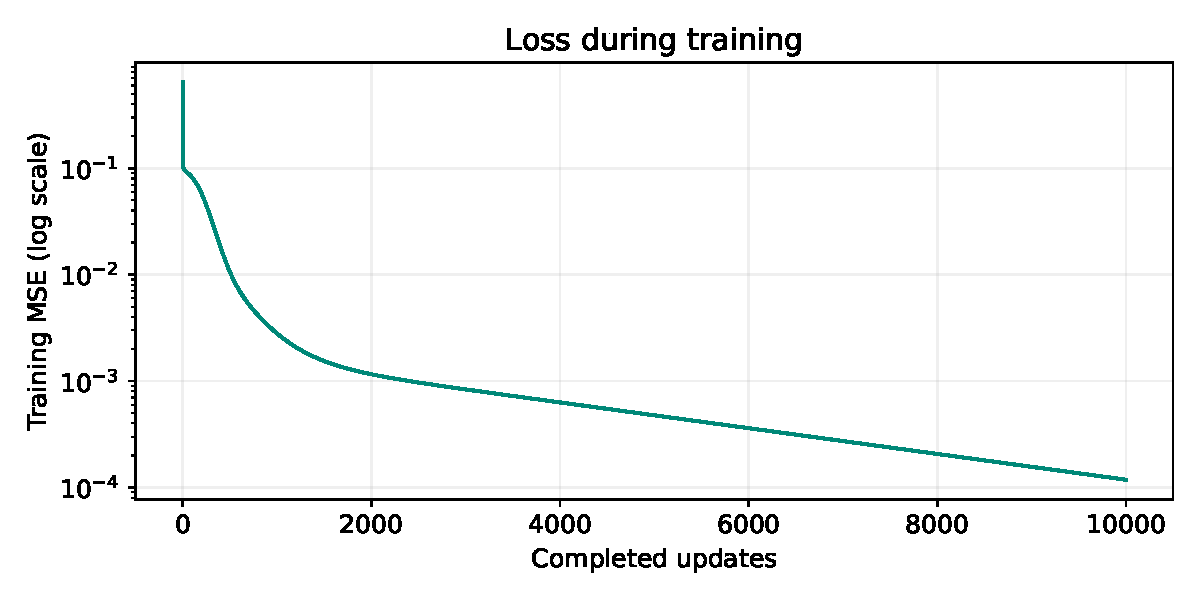
\includegraphics[width=0.79\textwidth,height=0.65\textheight,keepaspectratio]{figures/loss_curve.pdf}
\end{center}
\small
The vertical axis uses a logarithmic scale. Each stored loss precedes its update.\\
Final training MSE after 10,000 updates: $ 0.00011814 $.

\end{frame}

\begin{frame}{The learned curve approximates sine}
\begin{center}
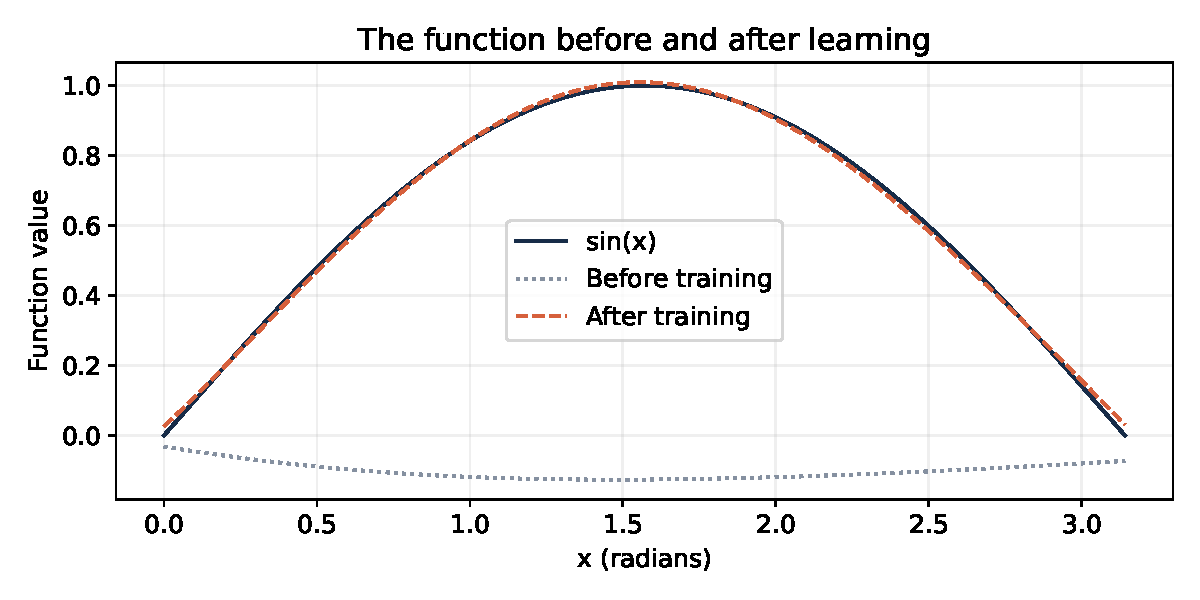
\includegraphics[width=0.81\textwidth,height=0.67\textheight,keepaspectratio]{figures/learned_function.pdf}
\end{center}
\small
Only the 49 parameters changed. The model evaluates sums of $\tanh$ terms.\\
We use sine to generate targets and compare results.
\end{frame}

\begin{frame}[fragile]{5. Testing on new inputs}
\begin{lstlisting}[basicstyle=\ttfamily\footnotesize]
x_test = torch.tensor(
    [0.1, 0.3, 0.6, 0.9, 1.2, 1.5]
).reshape(-1, 1)
y_test = torch.sin(x_test)
model.eval()
with torch.no_grad():
    y_pred = model(x_test)
error = (y_pred - y_test).abs()
test_mse = loss_fn(y_pred, y_test).item()
\end{lstlisting}
\vspace{2mm}
All six inputs lie in $[0,\pi/2]$ and differ from the training inputs.\\[2mm]
\texttt{no\_grad()} skips gradient tracking. No optimizer update occurs.
\end{frame}

\begin{frame}{Predictions compared with exact values}
\begin{center}
\small
\begin{tabular}{rrrr}
\toprule
$x$ (radians) & $\sin(x)$ & Prediction & Absolute error\\
\midrule
0.10 & 0.09983 & 0.11003 & 0.01019\\[1mm]
0.30 & 0.29552 & 0.28904 & 0.00648\\[1mm]
0.60 & 0.56464 & 0.55484 & 0.00980\\[1mm]
0.90 & 0.78333 & 0.78145 & 0.00188\\[1mm]
1.20 & 0.93204 & 0.93977 & 0.00774\\[1mm]
1.50 & 0.99749 & 1.00802 & 0.01053\\[1mm]
\bottomrule
\end{tabular}

\end{center}
\vspace{1mm}
Test MSE: $ 0.00006936 $\\[2mm]
Maximum absolute error at these six points: $ 0.01053 $.

\vspace{1mm}

\small Values come from the executed notebook. Table entries round to five decimal places.
\end{frame}

\begin{frame}{Small errors are easier to see separately}
\begin{center}
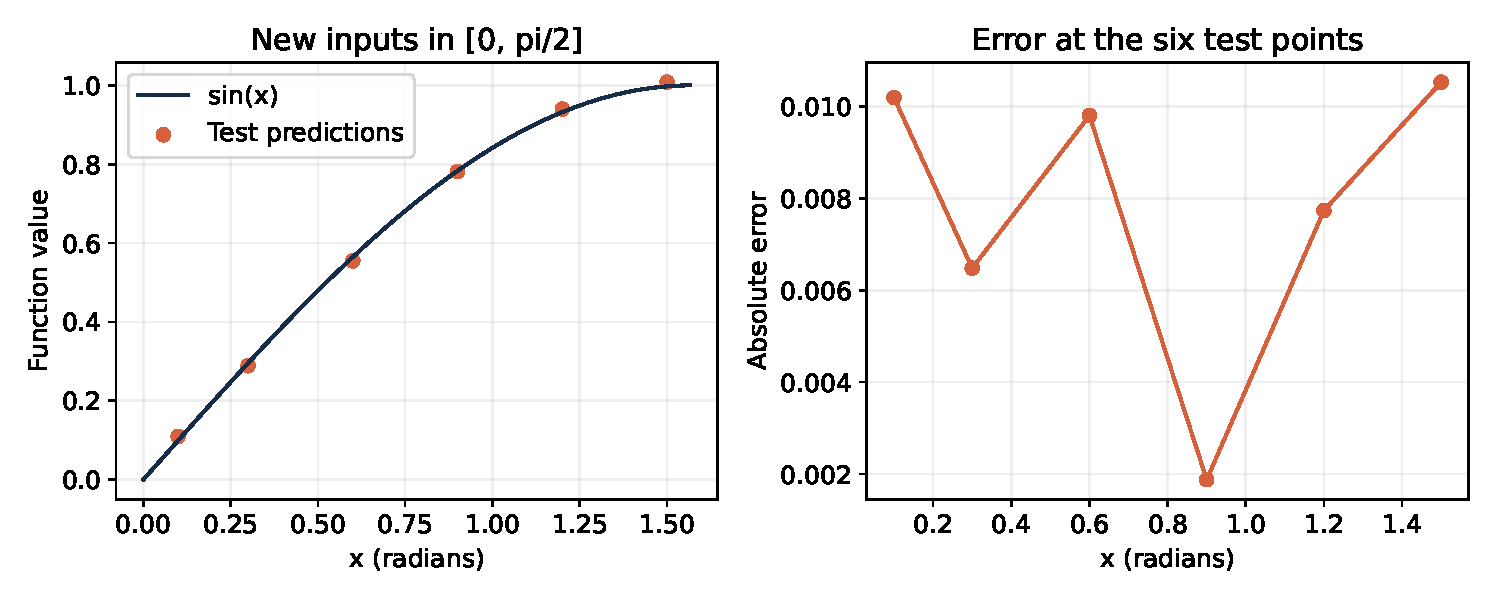
\includegraphics[width=\textwidth,height=0.66\textheight,keepaspectratio]{figures/test_results.pdf}
\end{center}
\small
Left: predictions against sine. Right: absolute error at the same six inputs.\\
Visual overlap alone does not mean the predictions are exact.
\end{frame}

\begin{frame}{What this experiment establishes}
\begin{itemize}\setlength\itemsep{5mm}
\item Training fits the sampled values by adjusting weights and biases.
\item The six new points check \alert{interpolation} inside the training interval.
\item Six points cannot establish accuracy everywhere in the interval.
\item The experiment does not establish accuracy beyond $[0,\pi]$ or teach periodicity explicitly.
\end{itemize}
\vspace{4mm}
If test results guide your choice of settings, reserve fresh test data for the final evaluation.
\end{frame}

\begin{frame}{Experiments for discussion}
\begin{enumerate}\setlength\itemsep{4mm}
\item Remove \texttt{nn.Tanh()}. What shape can the model learn?
\item Use 100 or 1,000 epochs. How does the fit change?
\item Use 4 hidden neurons instead of 16. Change both linear layers.
\item Plot on $[0,2\pi]$. Does the model reproduce the next half-wave?
\end{enumerate}
\vspace{5mm}
Restart the kernel and run all cells for each new experiment.
\vfill
\small\textcolor{Teal}{Companion notebook: \texttt{learning\_sine.ipynb}}\\[2mm]
\tiny Further reading: PyTorch \href{https://docs.pytorch.org/tutorials/beginner/basics/optimization_tutorial.html}{optimization} and
\href{https://docs.pytorch.org/tutorials/beginner/basics/autogradqs_tutorial.html}{automatic differentiation} tutorials.
\end{frame}

\end{document}
